\documentclass{article}
\usepackage{graphicx}
\usepackage{epstopdf}
\usepackage{float}
\usepackage{amsmath}
\usepackage{multicol}
%\usepackage{enumerate}
\usepackage{graphicx}
\usepackage{color}
\usepackage[utf8]{inputenc} 
\usepackage[portuguese]{babel}
\usepackage[font=normalsize,format=plain,labelfont=bf,up,textfont=up,figurename=Figura,tablename=Tabela]{caption}
\usepackage{subcaption}
\usepackage[top=1in, bottom=1in, left=1.25in, right=1.25in]{geometry}
\usepackage{indentfirst}
\usepackage{fancyhdr}

% Font packages
\usepackage{amssymb}
\usepackage{amsfonts}
\usepackage{steinmetz}
% Nice extra font package, e.g. \mathds{1}
\usepackage{dsfont}


% Use multiple rows when writing tables
\usepackage{multirow}
\usepackage{booktabs}
\usepackage{bigstrut}
    \setlength\bigstrutjot{3pt}

% Uncomment next line to make footnots per page
\usepackage{perpage}

% Uncoment next group of lines to create the table of contents for the PDF
\usepackage{hyperref}
\definecolor{darkblue}{rgb}{0,0,0.5}
\hypersetup{
    pdftitle={Título},
    pdfauthor={Lucas Canto},
    bookmarksnumbered=true,     
    bookmarksopen=true,         
    bookmarksopenlevel=1,       
    colorlinks=true,
    linkcolor=darkblue,
    filecolor=darkblue,  
    urlcolor=darkblue,  
    citecolor=darkblue,              
    pdfstartview=Fit,           
    pdfpagemode=UseOutlines,    % this is the option you were lookin for
    pdfpagelayout=TwoPageRight
}

\renewcommand{\title}{House Prices - Machine Learning}
\newcommand{\subtitle}{Tópicos Especiais em Sistemas de Controle}
\pagestyle{fancy}
\fancyhead[L]{\title}
\fancyhead[R]{\subtitle}
\fancyhead[C]{\thepage}
\fancyfoot[C]{}

\allowdisplaybreaks

\renewcommand{\labelitemi}{\scalebox{0.8}[0.8]{$\bullet$}}
\newcommand{\tab}{\hspace{0.5cm}}

\definecolor{lightyellow}{rgb}{1,0.9568,0.8039}
\definecolor{mygreen}{rgb}{0, 0.35, 0}
\definecolor{myblue}{rgb}{0,0,1}

\begin{document}
\large
\begin{titlepage}
\begin{center}

% Upper part of the page. The '~' is needed because \\
% only works if a paragraph has started.
\rule{\linewidth}{0.5mm}\\[0.4cm]
{\huge Universidade Federal do Rio de Janeiro}
\rule{\linewidth}{0.5mm}\\[0.4cm]
\vspace{5mm}

\includegraphics[width=0.3\textwidth]{../img/minerva3}~\\[1cm]

% Title
{ \huge \bfseries \title \\[0.4cm] }

\textsc{\Large \subtitle}\\[2cm]

% Author and supervisor
\begin{minipage}{0.4\textwidth}
\begin{flushleft} \large
{Aluno:\\ Lucas Gama Canto \\ DRE: 113114241 \\Id do Kaggle: lucascanto}\\
%NOME DOS ALUNOS

\end{flushleft}
\end{minipage}
\begin{minipage}{0.4\textwidth}
\begin{flushright} \large
{Professor:\\ Heraldo Luís Silveira de Almeida, D.Sc.}\\
%Professor
\end{flushright}
\end{minipage}

\vfill

% Bottom of the page
{\large \today}

\end{center}
\end{titlepage}

\section{Introdução}
	\paragraph{}Este trabalho se baseia na implementação de uma estratégia de aprendizado de máquina com o intuito de gerar uma estimativa do preço das casas da cidade de Ames, Iowa nos Estados Unidos. O problema partiu de uma competição do \textit{Kaggle} denominada \textit{House Prices: Advanced Regression Techniques} e além da composição deste relatório, a estimativa alcançada no final foi enviada ao site para que esta pudesse ser avaliada e alocada no rank da competição.
	
	\paragraph{}Este relatório irá abranger desde o pré-processamento dos parâmetros de treino e teste disponíveis no \textit{Ames Housing dataset}, fornecido pelo próprio Kaggle, até a escolha do método de validação cruzada, técnica de minimização de erro, treino e predição da variável alvo, ou seja, os preços das casas de Ames.
	
	\paragraph{}O código foi desenvolvido em \textit{python} e executado no \textit{Spyder}, utilizando bibliotecas de computação científica, machine learning e manipulação de dados como \textit{numpy}, \textit{pandas} e \textit{scikit-learn}.

\section{Pré-processamento de Dados}
	\paragraph{}O pré-processamento dos dados de treino e teste se mostram como uma importante etapa da implementação do aprendizado. A ideia é de tratar ou transformar estes dados de forma que estes se tornem mais propensos a serem analisados como variáveis dependentes do objetivo.
	
	\paragraph{}Como já informado, a variável objetivo no problema é o preço das casas, denominado nos dados de treino como SalePrice. As variáveis dependentes se resumem em valores numéricos e categóricos que representam atributos físicos, espaciais e geográficos da casa, estas informações variam desde a área em metros quadrados do porão e do primeiro andar da casa até o número de piscinas e qualidade geral do imóvel. Informações mais detalhadas sobre estas variáveis dependentes podem ser encontradas no arquivo \textit{data\_description.txt} fornecido pelo Kaggle. No total existem 80 variáveis dependentes à disposição de processamento.
	
	\paragraph{}A etapa de pré-processamento se dividiu em 5 etapas:
	\begin{itemize}
		\item Verificação de variáveis com maior correlação ao preço
		\item Remoção de \textit{Outliers}
		\item Preenchimento de dados nulos
		\item Normalização de variáveis
		\item Transformação de variáveis categóricas
	\end{itemize}
	
		\subsection{Matriz de Correlação}
			\paragraph{}De modo a limitar o espaço amostral e restringir algumas etapas do pré-processamento apenas à variáveis que possuam uma relação mais direta à variável objetivo, a matriz de correlação das variáveis dependentes em relação ao preço foi analisada.
			
			\begin{figure}[h]
				\centering
				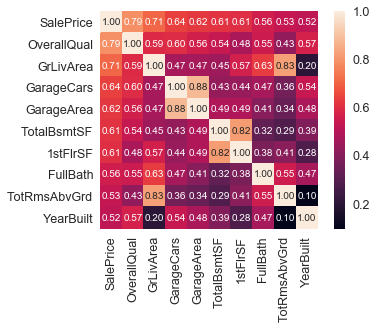
\includegraphics[scale=0.9]{../img/correlation}
				\caption{Matriz de correlação das 10 variáveis mais correlatas a SalePrice}
			\end{figure}
			
			\paragraph{}É possível verificar que quase todas as variáveis verificadas como as mais correlatas se apresentam como numéricas, com a exceção de \textit{OverallQual} que coincidentemente também se apresentou como a variável mais correlata.
			
			\paragraph{}Como \textit{OverallQual} se trata de uma variável categórica, esta variável não irá ser modificada nas etapas de relação de outliers e normalização, visto que isto poderia acarretar na perda de possíveis dados importantes para o treino da estratégia.
			
			\paragraph{}Outro fator a ser analisado é a semelhança de valores de correlação entre variáveis dependentes, isto indica que não há necessidade de utilizar duas variáveis com o mesmo grau de correlação pois elas possivelmente tem um comportamento semelhante perante a variável objetivo. Pares de variáveis como \textit{GarageCars} e \textit{GarageArea}, \textit{TotalBsmtSF} e \textit{1stFloor}, \textit{TotRmsAbvGrd} e \textit{GrLivArea} se encaixam nessa característica.
			
		\subsection{Remoção de Outliers}
			\paragraph{}Baseado na decisão da seção anterior de utilizar apenas as variáveis com maior correlação em relação ao preço das casas, foram selecionadas as seguintes variáveis para a avaliação de outliers: \textit{OverallQual}, \textit{GrLivArea}, \textit{GarageCars}, \textit{TotalBsmtSF}, \textit{FullBath} e \textit{YearBuilt}.
			
			\paragraph{}O plot bivariável de cada variável escolhida foi gerado junto a \textit{SalePrice} e este foi analisado.
		
			\begin{figure}[H]
				\centering
				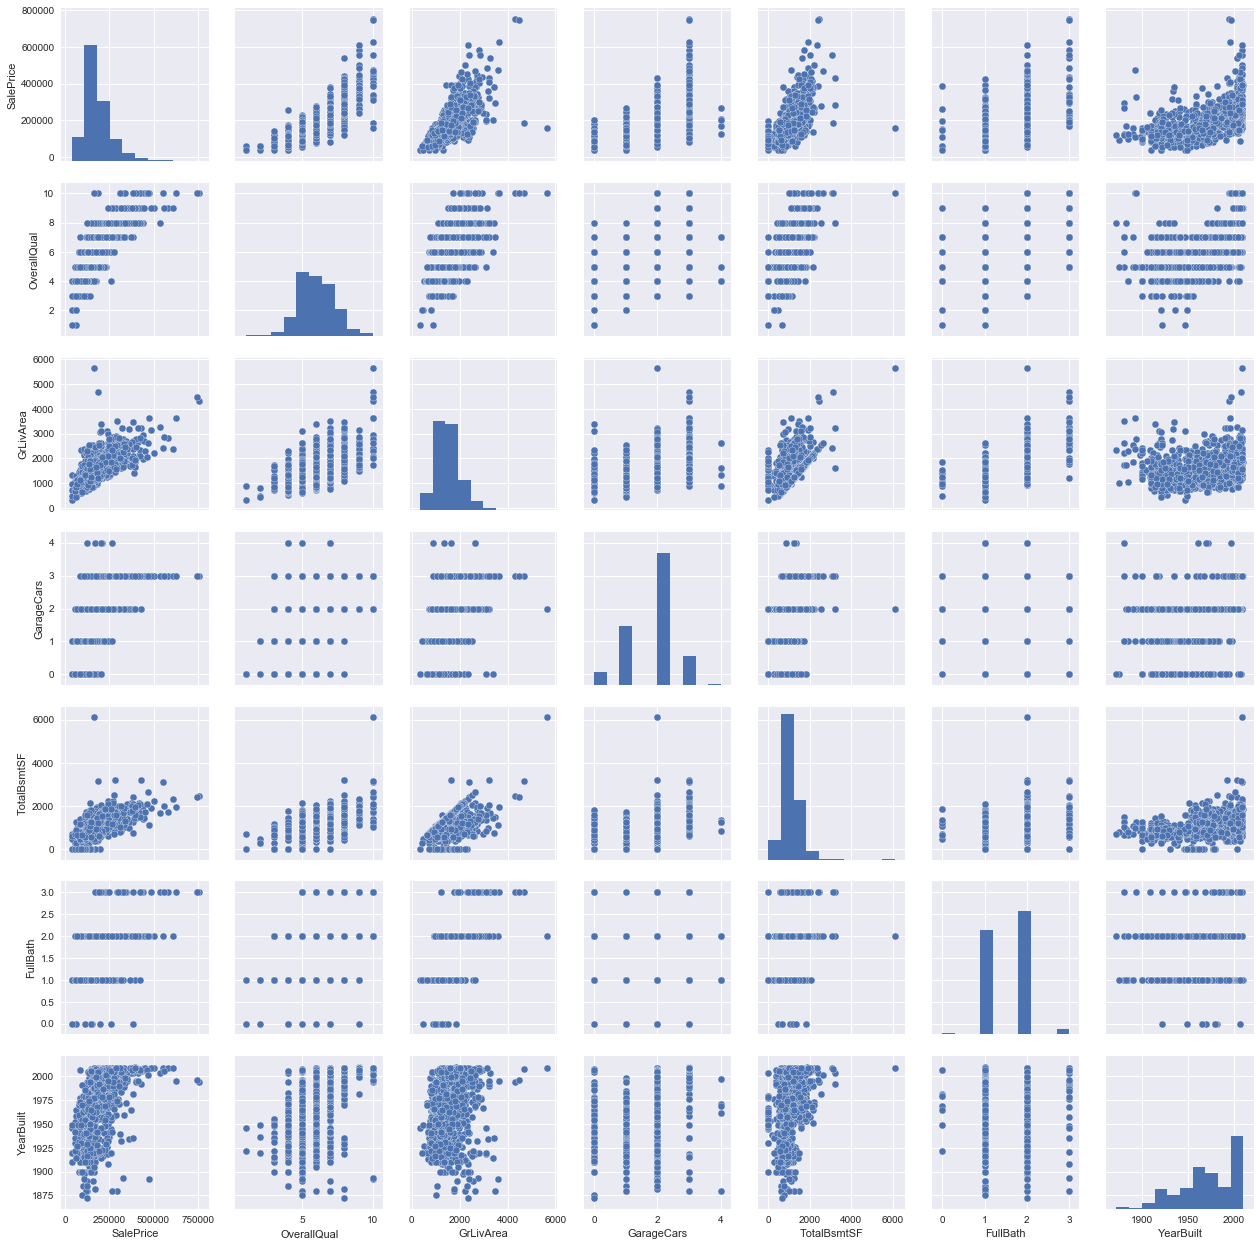
\includegraphics[scale=0.35]{../img/scatter}
				\caption{\textit{Scatter plot} das variáveis selecionadas}
			\end{figure}
		
			\paragraph{}Podemos observar que existem possíveis outliers nas variáveis \textit{GrLiveArea} e \textit{TotalBsmtSF}. Há também alguns dados que podem ser considerados outliers em \textit{YearBuilt}, mas a remoção deste resultou em grande perda de informação e consequentemente numa previsão menos performática. Sendo assim, a remoção dos outliers foi feita apenas nas duas primeiras variáveis mencionadas.
		
			\paragraph{}Em \textit{GrLiveArea}, houveram pontos de grande valor de área de convivência com baixo preço. Estes pontos podem significar valores de casas que se encontram numa área rural da cidade, mas foram considerados outliers por sua baixa frequência.
			\begin{figure}[H]
				\centering
				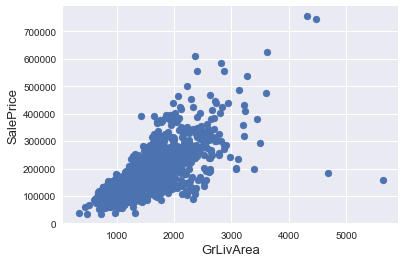
\includegraphics[scale=0.8]{../img/grlivearea_outliers}
				\caption{Os dois pontos na extrema direita inferior foram considerados outliers.}
			\end{figure}
		
			\begin{figure}[H]
				\centering
				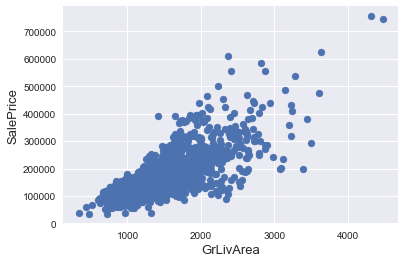
\includegraphics[scale=0.8]{../img/grlivearea_no_outliers}
				\caption{Plot após a remoção dos outliers.}
			\end{figure}
			
			\paragraph{}Para \textit{TotalBsmtSF}, alguns pontos foram visualmente considerados outliers por não seguirem o fluxo de outros pontos do dataset.
			
			\begin{figure}[H]
				\centering
				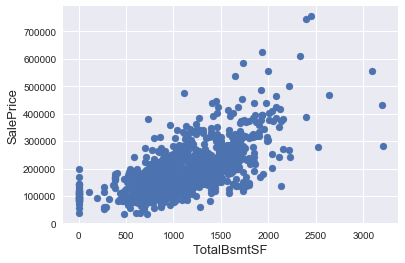
\includegraphics[scale=0.8]{../img/totalbsmtsf_outliers}
				\caption{Os três pontos na extrema direita foram considerados outliers no caso de \textit{TotalBsmtSF}.}
			\end{figure}
			
			\begin{figure}[H]
				\centering
				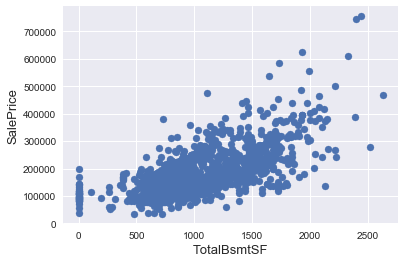
\includegraphics[scale=0.8]{../img/totalbsmtsf_no_outliers}
				\caption{Plot após a remoção dos outliers.}
			\end{figure}
		
		\subsection{Preenchimento de Dados Nulos}
			\paragraph{}Algumas amostragens, tanto no dataset de treino quanto no dataset de teste, apresentavam valores nulos em algumas variáveis dependentes, fazendo com que fosse necessário um tratamento desses dados antes de utiliza-los no algoritmo de treino.
			
			\paragraph{}A técnica utilizada em todos os valores nulos que existiam em ambos os datasets foi o \textit{Foward Fill} disponível no pacote \textit{pandas}. Esta técnica consiste em preencher um valor vazio a partir de um valor preenchido em uma amostragem anterior, fazendo com que ocorra uma continuidade entre pontos. 
		
			\begin{figure}[H]
				\centering
				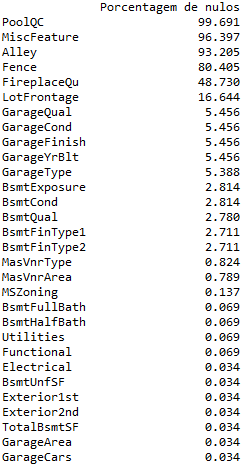
\includegraphics[scale=0.9]{../img/null_data}
				\caption{Porcentagem de dados nulos no dataset de treino e teste concatenados.}
			\end{figure}
		
			\paragraph{}Porém, em alguns casos, como para as variáveis \textit{PoolQC}, \textit{MiscFeature}, \textit{Alley} e \textit{Fence}, que apresentam uma alta porcentagem de valores nulos, esta técnica não se mostra tão promissora pois a repetição dos únicos dados existentes pode causar um certo vício na curva a ser aproximada através destes dados.
		
		\subsection{Normalização de Variáveis}
			\paragraph{}Como em tese, os dados devem se assemelhar a uma distribuição normal porque testes estatísticos contam com isto, foi aplicada uma transformação logarítmica para que sua assimetria fosse diminuída.
			
			\paragraph{}No caso de \textit{SalePrice}, por sua ausência no dataset de teste, a normalização ocorreu apenas no dataset de treino.
			
			\begin{figure}[H]
				\centering
				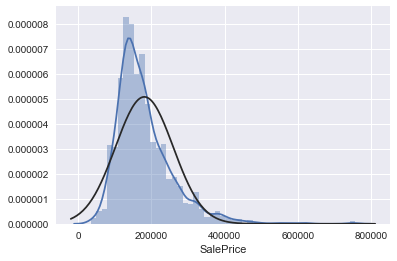
\includegraphics[scale=0.8]{../img/saleprice_norm_1}
				\caption{Histograma de \textit{SalePrice}}
			\end{figure}

			\begin{figure}[H]
				\centering
				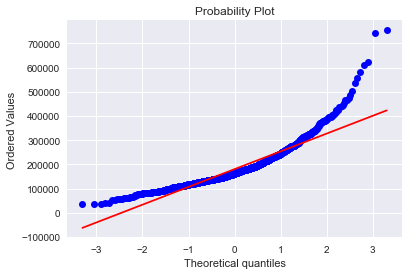
\includegraphics[scale=0.8]{../img/saleprice_norm_2}
				\caption{Distribuição de probabilidade de \textit{SalePrice}}
			\end{figure}
			
			\begin{figure}[H]
				\centering
				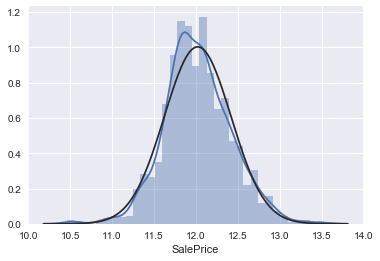
\includegraphics[scale=0.8]{../img/saleprice_norm_after_1}
				\caption{Histograma de \textit{SalePrice} após a transformação}
			\end{figure}
			
			\begin{figure}[H]
				\centering
				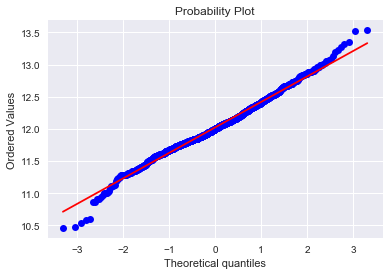
\includegraphics[scale=0.8]{../img/saleprice_norm_after_2}
				\caption{Distribuição de probabilidade de \textit{SalePrice} após a transformação}
			\end{figure}
			
			\paragraph{}De forma semelhante, mas para os datasets concatenados, a normalização de \textit{GrLivArea} também foi feita através de transformação logarítmica.
			
			\begin{figure}[H]
				\centering
				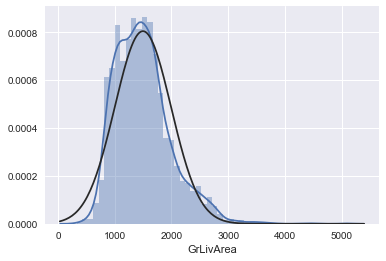
\includegraphics[scale=0.8]{../img/grlivearea_norm_1}
				\caption{Histograma de \textit{GrLivArea}}
			\end{figure}
			
			\begin{figure}[H]
				\centering
				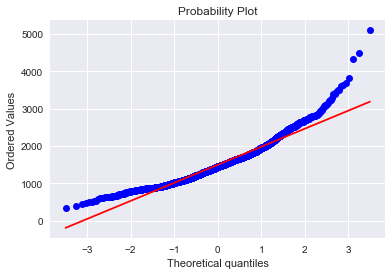
\includegraphics[scale=0.8]{../img/grlivearea_norm_2}
				\caption{Distribuição de probabilidade de \textit{GrLivArea}}
			\end{figure}
			
			\begin{figure}[H]
				\centering
				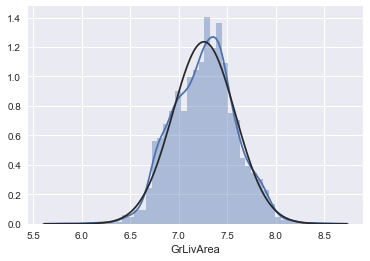
\includegraphics[scale=0.8]{../img/grlivearea_norm_after_1}
				\caption{Histograma de \textit{GrLivArea} após a transformação}
			\end{figure}
			
			\begin{figure}[H]
				\centering
				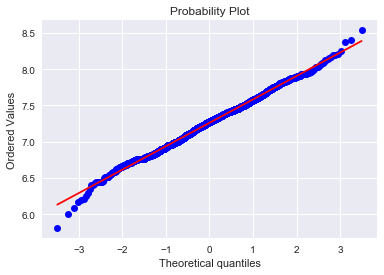
\includegraphics[scale=0.8]{../img/grlivearea_norm_after_2}
				\caption{Distribuição de probabilidade de \textit{GrLivArea} após a transformação}
			\end{figure}
			
			\paragraph{}Por ter muitos valores iguais a zero, significando casas sem porão, a transformação logarítmica na variável \textit{TotalBsmtSF} foi feita em todos os pontos menos os pontos com \textit{TotalBsmtSF} iguais a zero.
			
			\begin{figure}[H]
				\centering
				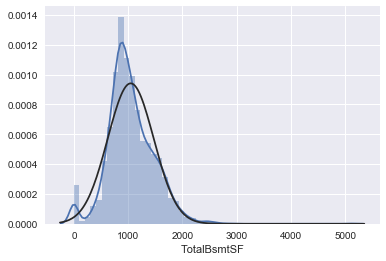
\includegraphics[scale=0.8]{../img/totalbsmtsf_norm_1}
				\caption{Histograma de \textit{TotalBsmtSF}}
			\end{figure}
			
			\begin{figure}[H]
				\centering
				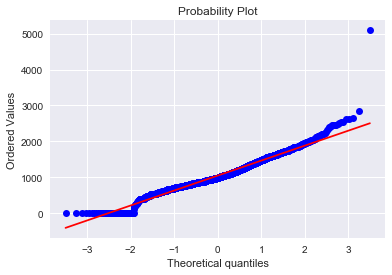
\includegraphics[scale=0.8]{../img/totalbsmtsf_norm_2}
				\caption{Distribuição de probabilidade de \textit{TotalBsmtSF}}
			\end{figure}
			
			\begin{figure}[H]
				\centering
				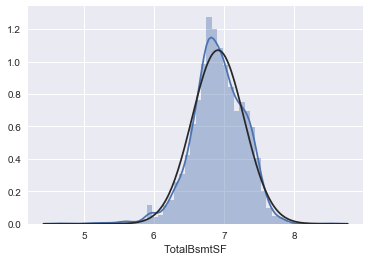
\includegraphics[scale=0.8]{../img/totalbsmtsf_norm_after_1}
				\caption{Histograma de \textit{TotalBsmtSF} após a transformação}
			\end{figure}
			
			\begin{figure}[H]
				\centering
				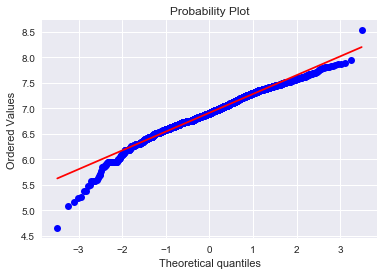
\includegraphics[scale=0.8]{../img/totalbsmtsf_norm_after_2}
				\caption{Distribuição de probabilidade de \textit{TotalBsmtSF} após a transformação}
			\end{figure}						
						
		\subsection{Transformando Variáveis Categóricas}
			\paragraph{}As variáveis categóricas foram transformadas em \textit{dummies} utilizando um método com este objetivo específico do pacote \textit{pandas}.
			
			\paragraph{}Este método faz com que cada categoria de cada variável categórica se transforme em uma nova coluna no dataset, isto é, uma nova variável dependente onde é possível apenas ter o valor atribuído com 0 ou 1 (falso ou verdadeiro). As colunas que comportavam as variáveis categóricas são substituídas pelas \textit{dummies} que representam suas categorias no dataset.
		
		
\section{Treinamento e Previsão}
	\paragraph{}Após o pré-processamento dos dados, a função de validação cruzada foi definida utilizando desvio médio quadrado (RMSE).

	\paragraph{}O dataset resultante da concatenação dos dados de treino e teste foram novamente separados e o dataset de treino foi treinado utilizando o pacote \textit{LightGBM} da Microsoft que se resume em um framework que utiliza um método rápido e de alta performance de descida de gradiente para otimização.
	
	\paragraph{}Um score a partir da comparação entre os preços previstos pelas variáveis dependentes no dataset de treino e os preços do mesmo dataset foi levantado e obteve o valor de $0.1153 (0.0088)$, este valor não foi considerado alto e foi importante para mostrar que possivelmente o modelo gerado não estava com \textit{overfitting}, o que ocasionaria num ótimo desempenho no dataset de treino mas um desempenho ruim no dataset de teste.
	
	\paragraph{}Utilizando o modelo levantado, os preços das casas com as características citadas no dataset de teste foram previstos e gravados no arquivo \textit{submission.csv} e este foi enviado ao Kaggle para apuração.
\section{Conclusão}

	\paragraph{}Após o envio da previsão para o Kaggle, o rank atribuído ao modelo enviado foi a colocação de $885/4803$, que tardiamente caiu para $888/4803$ e pode ser que caia ainda mais no futuro diante da alta competitividade da competição.
	
	\paragraph{}Ainda assim, foi possível se alocar dentre a porcentagem dos $19\%$ melhores da competição, o que foi pessoalmente satisfatório.
	
	\paragraph{}Para futuras melhorias e reflexões em projetos semelhantes, pode-se argumentar que algumas acochambrações poderiam ter sido evitadas em algumas etapas do processo.
	
	\paragraph{}Por exemplo, o  método utilizado para o preenchimento de dados vazios foi genérico e generalista, o que negligenciou uma possível melhora de desempenho ao não tratar cada caso de variável independente de forma isolada. Algumas outras técnicas estatísticas, como a transformação \textit{Box Cox} em variáveis de distribuição menos uniformes também foram deixadas de lado, o que poderia substancialmente aumentar o desempenho do modelo gerado.
	
	\begin{figure}[H]
		\centering
		
\includegraphics[scale=0.6]{../img/final_score}
		\caption{Score final almejado no site do Kaggle.}
	\end{figure}

\end{document}